\chapter{Research Goals}
\label{cha:ResearchGoals}

The goal of this thesis is to contribute in the domain of autonomous driving by investigating the use of \ac{RL} to train an autonomous driving agent that is resilient to changes in light conditions. The agent is evaluated on simulated tracks that consist of a series of goals indicated by two blocks, a tracks is successfully completed if the agents drives through all goals in order \ref{fig:track_and_agent}.
This thesis builds upon previous work at the ScaDS.AI \textcite{maximilian} and uses the same tracks and task specifications. The agent from previous work was not able to reliably complete tracks under changing light conditions, motivating the research goals.


The agent and the policy are designed to be resilient to light changes. To achieve this, the policy is trained using \ac{RL} in a simulated environment with changing light conditions. The policy consists of a \ac{CNN}, the inputs to the \ac{CNN} are camera images from the perspective of the agent \ref{fig:track_and_agent}. Preprocessing steps are applied to the camera images to improve the performance of the policy under changing light conditions. The policy is trained end-to-end using an \ac{RL} algorithm. This allows the policy to learn the relevant features from the camera images itself.
Different training approaches and preprocessing steps to develop a powerful agent are investigated.


\begin{figure}
    \centering
    \subfigure{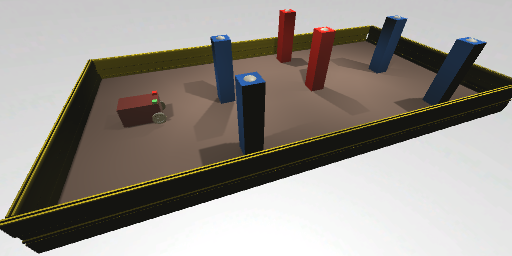
\includegraphics[width=0.4\textwidth]{Bilder/image_printer_images/evaluation_hard.png}}\qquad
    \subfigure{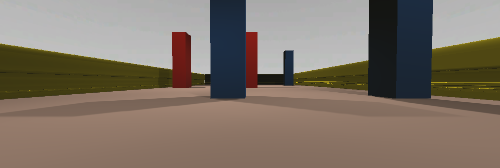
\includegraphics[width=0.4\textwidth]{Bilder/image_printer_images/agent_image_from_unity.png}}\\
    \caption{Example image of a track and the agent's camera}
    \label{fig:track_and_agent}
\end{figure}


\section{Question 1 - \questionOne}

The previous work by \textcite{maximilian} showed that it is possible to train an agent using \ac{RL} to solve the evaluation tracks, however the trained agents were not successful in reliably traversing the tracks of higher difficulty levels. The agents developed in previous work utilized an extensive preprocessing pipeline to extract the relevant information from the camera images for processing by the policy. The evaulation by \textcite{merlin_flach} showed that the preprocessing pipeline's performance depends heavily on the light settings of the environment.

This thesis will use a \ac{CNN} network policy that is trained end-to-end using \ac{RL}. It has already been shown to be possible to train an agent to solve the autnomous driving task using \ac{RL}. However the agents developed in previous work used different preprocessing steps and policies compared to the agents developed here.

Due to these differences in implementation and as a prerequisite for question 2 and 3, it is first important to investigate if it is possible to train a \ac{CNN} policy to reliably solve the tracks of all difficulty levels. This raises question 1:
\questionOne

The question will be answered by developing agents based on related work. The training process of the agents will use common practices from \ac{RL} adapted to the specific task. The developed agent's $success\_rate$ and $collision\_rate$ will be evaluated on all difficulty settings to answer the question.


\section{Question 2 - \questionTwo}

Question 1 investigates if it is possible to develop a successful \ac{CNN}-based agent solving the tracks of all difficulty levels. 
Question 2 then investigates if it is possible to make the \ac{CNN}-based agents robust to changing light conditions.

The agents developed for question 1 will be used as a basis for the agents developed in this question. The agents will be augmented with preprocessing steps that improve the performance of the agents under changing light conditions. These preprocessing steps will be applied to the camera images before they are processed by the policy. The agent's policy will be trained in a simulated environment with changing light conditions to help the agent generalize and learn.

Similarly the $success\_rate$ and $collision\_rate$ will be primarily used to evaluate and compare the agent's performance. The performance difference between different light conditions will be used to answer the question. If the performance for all light conditions is comparable to the performance of agents in question 1, the agents can be considered robust to changing light conditions.

\section{Question 3 - \questionThree}

One goal of the ongoing research at the ScaDS.AI is to build physical robots for demonstration and research purposes \textcite{merlin_flach}. The robots are based on the NVIDIA JetBot platform \autocite{jetbot}. They are equiped with a camera, wheels and a small on-board computer. A future goal is to transfer trained policies onto these robots and execute them in real-life. However the limited processing power of these robots might not be sufficient for more complex agents that utilize \acp{NN}. This raises question 3 - \questionThree


The question will be answered by investigating the processing power required to run the preprocessing steps and \acp{NN} used in the agents. This will be evaluated empirically by creating recordings of the agents in simulations. The recordings are then replayed on the physical hardware. The evaluation checks if the physical hardware is able to reproduce the preprocessing steps and policy from the replays in real-time.

